\documentclass[10pt,a4paper]{article}
\usepackage[utf8]{inputenc}
\usepackage{amsmath}
\usepackage{amsfonts}
\usepackage{amssymb}
\usepackage{graphicx}
\begin{document}
\section{Johdanto}
\subsection{Ohjelman kuvaus}
Tarkoitus on toteuttaa web-sovellus, joka mahdollistaa tiedostojen lataamisen palvelimelle ja palvelimelta. Palvelimella olevia tiedostoja voi kommentoida. Tiedostoihin liittyy myös teemasanoja, joiden perusteella tiedostoja voi hakea. Käyttäjät voivat rekisteröityä palveluun, mutta se ei ole pakollista. Kaikki käyttäjät voivat lisätä tiedostoja ja viestejä. Rekisteröityneet käyttäjät voivat lisäksi muokata tai poistaa lisäämiään tiedostoja tai viestejä.

\subsection{Toteutus- ja toimintaympäristö}
Sovellus toteutetaan PHP:llä ja se toimii Helsingin yliopiston users-palvelimella. Sovellus käyttää PostgreSQL-tietokantaa.

\section{Käyttötapaukset}
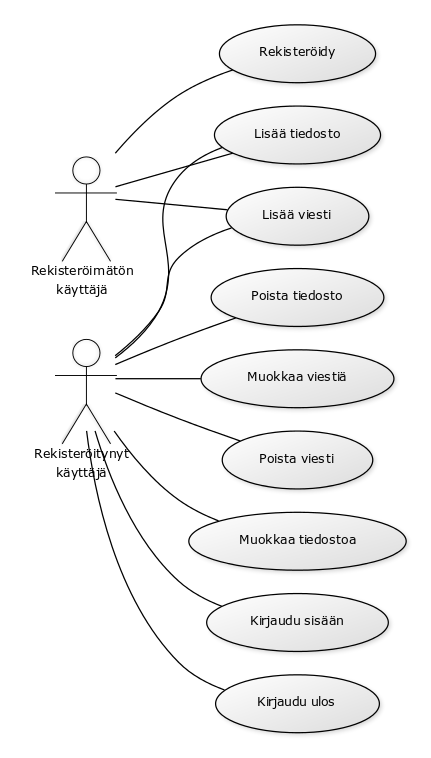
\includegraphics[scale=0.7]{kaaviot/kayttotapauskaavio.png}


\subsection{Rekisteröimättömän käyttäjän käyttötapaukset}
\subsubsection{Lisää tiedosto}
Käyttäjä lisää tiedoston palvelimelle.
\subsubsection{Lisää viesti}
Käyttäjä lisää viestin johonkin tiedostoon liittyen.

\subsubsection{Rekisteröidy}
Luodaan käyttäjälle käyttäjätunnus. Tämän jälkeen käyttäjä voi kirjautua järjestelmään.
\subsubsection{Kirjaudu sisään}
Käyttäjä tunnistautuu järjestelmään.


\subsection{Rekisteröityneen käyttäjän käyttötapaukset}
\subsubsection{Lisää tiedosto}
Käyttäjä lisää tiedoston palvelimelle.
\subsubsection{Muokkaa tiedostoa}
Tiedostoon liittyvää metatietoa, kuten nimeä tai kuvausta, voi muokata. Tiedoston sisältöä ei voi muokata.
\subsubsection{Poista tiedosto}
Käyttäjän valitsema ja omistama tiedosto poistetaan. Tiedostoon liittyvät viestit ja metatiedot poistetaan myös.

\subsubsection{Lisää viesti}
Käyttäjä lisää viestin johonkin tiedostoon liittyen.
\subsubsection{Muokkaa viestiä}
Rekisteröitynyt käyttäjä voi muokata minkä tahansa lähettämänsä viestin sisältöä, aihetta tai muita tietoja.
\subsubsection{Poista viesti}
Käyttäjän valitsema ja omistama viesti poistetaan.

\subsubsection{Kirjaudu ulos}
Käyttäjä kirjataan ulos.
\end{document}
